\documentclass{article}
\usepackage{tikz, comment}
\usepackage{pifont}
\usepackage{fontspec}
\usetikzlibrary{arrows, decorations.markings, decorations.pathreplacing}
\begin{comment}
:Title: Not defined yet
:Tags: focus of a parabola;parabola;directrix of a parabola;tangent line;focal radius 
:Prob: 0.5351;0.5339;0.5245;0.5087;0.4892
:Author: Prof.Hu Ji-shan, HKUST
:Slug: No name yet

Description Here.........
\end{comment}
\begin{document}\centering

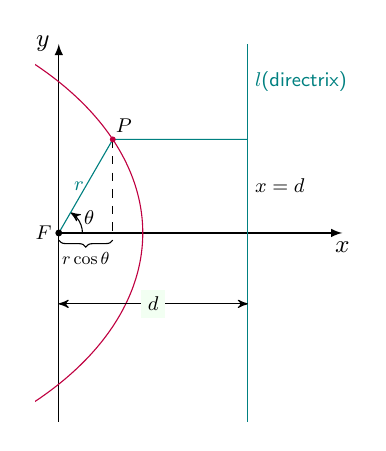
\begin{tikzpicture}[>=latex,xscale=.5*0.6, yscale=.5*0.6][font=\sf\small]

\draw[->] (0, 0) -- (12, 0)node[below] {\small $x$};
\draw[->] (0, -8) -- (0, 8)node[left] {\small $y$};

\clip[] (-1,-8) rectangle (12.2, 8);

\draw[purple, samples=100, smooth, domain=-pi/2-1:pi/2+1, variable=\t]
plot ({0.8*8/(1+0.8*cos(\t r))*cos(\t r)}, {0.8*8/(1+0.8*cos(\t r))*sin(\t r)}) ;

\draw[->, >=stealth', samples=7, smooth, domain=0:pi/3, variable=\t]
plot ({1*cos(\t r)}, {1*sin(\t r)});
\node[xshift=11, yshift=5.5, scale=0.8] at (0,0) {$\theta$};

\draw[dashed] ({0.8*8/(1+0.8*cos(60))*cos(60)}, {0.8*8/(1+0.8*cos(60))*sin(60)}) -- ({0.8*8/(1+0.8*cos(60))*cos(60)}, 0);

\draw[teal] (8, -8) -- (8, 8) node[right, pos =0.9, scale=0.8] {$l$($\hbox{directrix}$)};

\draw[teal] (0,0)--({0.8*8/(1+0.8*cos(60))*cos(60)}, {0.8*8/(1+0.8*cos(60))*sin(60)}) node[left, xshift=2, pos=0.5, scale=0.8]{$r$} --(8, {0.8*8/(1+0.8*cos(60))*sin(60)}) ;

\draw[purple, fill, xscale=1/0.6, yscale=1/0.6] ({0.8*8/(1+0.8*cos(60))*cos(60)*0.6}, {0.8*8/(1+0.8*cos(60))*sin(60)*0.6}) circle(0.06) node[black, above, xshift=4, scale=0.8] {$P$};
\draw[fill, xscale=1/0.5, yscale=1/0.5] (0, 0) circle(0.06) node[left, scale=0.8]{$F$};

\node[right, scale=0.8] at (8, 2) {$x=d$};

\draw [decoration={brace,raise=2, mirror},decorate, yshift=-2]
(0, 0) -- ({0.8*8/(1+0.8*cos(60))*cos(60)}, 0) node[black, below, midway, pos=0.5, xshift=0, yshift=-4, scale=0.7]{$r\cos \theta$};

\draw[<->, >=stealth'] (0, -3) -- (8, -3) node[pos=0.5, fill=green!5!white, scale=0.8] at (8, 2) {$d$};

\end{tikzpicture}
\end{document}